% Chapter: Methods (file renamed from methodology.tex 2026-08-03)
% Reaction-diffusion excitable media as substrates for analog physical computation
% SHORTENED COPY-EDIT (Report/edits/, 2026-08-03): prose paragraphs tightened.
% Original untouched at chapters/methodology.tex.

\section{Overview}
\label{sec:meth_overview}

The methodology of this thesis follows a characterise-before-train philosophy: before asking how a structured excitable medium might be optimised for a computational task, we first measure, in a controlled and reproducible way, what the unoptimised medium already does.
It has three layers.
The model layer describes the Belousov--Zhabotinsky (BZ) medium by two-variable reaction-diffusion kinetics, extended with three substrate parameterisations - wall geometry, a light-suppression field, and an anisotropic diffusion tensor - that act as the candidate ``weights'' of the substrate.
The solver layer is an explicit finite-difference scheme with adaptive reaction subcycling, verified against known excitable-media phenomenology and convergence-tested in space and time.
The protocol layer is a black-box characterisation: the substrate is stimulated at defined input ports and its response recorded at fixed probes, yielding transfer functions rather than snapshots.
Two kinetics are paired throughout: the Barkley model \cite{barkley1991model}, a computationally cheap literature-standard workhorse used for the headline measurements, and the chemically grounded Oregonator model \cite{field1974oregonator, tyson1980target}, used to corroborate them.
Agreement between two kinetics with different mathematical structure and different physical provenance is taken as evidence that a measured transfer function is a property of excitable media generally, rather than an artefact of one model's parameterisation.

\section{The Oregonator Model}
\label{sec:meth_oregonator}

\subsection{Two-Variable Reduction}
\label{sec:meth_oregonator_2var}

The chemical basis of the substrate is the BZ reaction, modelled by the two-variable Tyson--Fife reduction of the Oregonator introduced in \refSec{sec:lit_bz} \cite{field1974oregonator, tyson1980target}.
In the scaled Tyson-Fife form used throughout this thesis, the kinetics of the activator $u$ and recovery variable $v$ are:
\begin{equation}
\frac{\partial u}{\partial t} = \frac{1}{\varepsilon}\left[\,u - u^{2} - \left(f v + \phi\right)\frac{u - q}{u + q}\,\right] + \nabla\!\cdot\!\left(\mathbf{D}\,\nabla u\right),
\label{eq:oregonator_u}
\end{equation}
\begin{equation}
\frac{\partial v}{\partial t} = u - v + D_{v}\,\nabla^{2} v,
\label{eq:oregonator_v}
\end{equation}
where $u$ represents the scaled concentration of the autocatalytic activator species HBrO$_{2}$, $v$ the scaled concentration of the oxidised metal catalyst, and $\phi$ the intensity of illumination in the photosensitive ruthenium-catalysed variant of the reaction, in which light produces bromide and thereby suppresses excitability \cite{sakurai2002design}.
The parameter $\varepsilon \ll 1$ sets the timescale separation between the fast activator and the slow recovery dynamics, $f$ is a stoichiometric factor controlling the position of the rest state and hence the excitability, and $q \ll 1$ is a small scaling ratio.
This singularly perturbed structure - a fast excitation variable with a cubic-like nullcline and a slow linear recovery variable - is what gives the medium its excitable pulse dynamics \cite{tyson1988singular}.

Alongside the Oregonator, the Barkley model \cite{barkley1991model} is used as a phenomenological alternative designed explicitly for fast simulation of excitable-media phenomenology:
\begin{equation}
\frac{\partial u}{\partial t} = \frac{1}{\varepsilon}\,u\left(1 - u\right)\left(u - \frac{v + b}{a}\right) + D_{u}\,\nabla^{2}u,
\qquad
\frac{\partial v}{\partial t} = u - v.
\label{eq:barkley}
\end{equation}
The Barkley kinetics retain the essential structure of an excitable medium but replace the Oregonator's rational nonlinearity with polynomial terms, eliminating the division by $u + q$ and the associated numerical stiffness near $u = 0$.
The parameters used here are $a = 0.75$, $b = 0.01$, $\varepsilon = 0.02$, $D_{u} = 1$, and $D_{v} = 0$, a standard excitable parameter set from the literature.
Because \refeqn{eq:barkley} carries no chemical interpretation of its parameters, it serves purely as a fast workhorse; every headline result measured with it is cross-checked against the Oregonator, whose parameters map onto identifiable chemical rates.

\subsection{Physical Units and Scaling}
\label{sec:meth_scaling}

The dimensionless variables of \refeqn{eq:oregonator_u}-\refeqn{eq:oregonator_v} are defined rescalings of physical concentrations, and the rescaling factors are known for a reference BZ recipe \cite{tyson1980target}.
In the Tyson--Fife scaling,
\begin{equation}
u = \frac{2 k_{4}}{k_{3} A}\,[\mathrm{HBrO_{2}}],
\qquad
v = \frac{k_{c} k_{4} B}{(k_{3} A)^{2}}\,[\mathrm{Ce(IV)}],
\qquad
\tau = k_{c} B\,t,
\label{eq:tyson_fife_scaling}
\end{equation}
where $t$ is physical time, $\tau$ the model time, and $A = [\mathrm{BrO_{3}^{-}}]$ and $B = [\mathrm{malonic\ acid}]$ the concentrations of the bath species.
With the acidity-adjusted FKN rate constants at $[\mathrm{H}^{+}] = 0.8$ M ($k_{1} = 1.28$, $k_{2} = 2.4 \times 10^{6}$, $k_{3} = 33.6$, $k_{4} = 2400$ M$^{-1}$s$^{-1}$, $k_{c} = 1$ M$^{-1}$s$^{-1}$) \cite{field1986oxybromine}
and the reference composition $A = 0.06$ M, $B = 0.02$ M, the time scaling is $\tau = 0.02\,t$ with $t$ in seconds: one model time unit corresponds to about 50 s, though the exact factor is recipe-dependent, since $k_{c}$, $B$, and the acidity all shift it.
The length unit follows from the activator diffusivity: with $D \approx 2 \times 10^{-5}$ cm$^{2}$s$^{-1}$ and a 50 s time unit, $L_{0} = \sqrt{D T_{0}} \approx 0.3$ mm, so one grid cell at the working resolution corresponds to about 0.3 mm.
As a cross-check, the measured model pulse speed of 6.2 cells per time unit (\refSec{sec:meth_regime}) maps to about 0.04 mm/s, within a factor of about four of the 0.15 to 0.2 mm/s pulse speeds measured in photosensitive BZ layers \cite{suematsu2021instability}, the level of agreement expected given the recipe dependence of both numbers.

This mapping is a calibration, not an identity.
The FKN-fitted canonical dimensionless parameters of the scaling are $\varepsilon = k_{c} B / (k_{3} A) = 9.9 \times 10^{-3}$ and $q = 2 k_{1} k_{4} / (k_{2} k_{3}) = 7.6 \times 10^{-5}$, whereas every simulation in this thesis uses the computational parameter set $\varepsilon = 0.05$, $q = 0.002$, $f = 1.4$, the standard choice in the wave-simulation literature because it preserves the pulse dynamics while giving convenient numerics.
The SI figures in this subsection should therefore be read as an order-of-magnitude calibration against a typical recipe, not as an exact conversion of the model's units.

For the substrate, the mapping sets the physical scale of every measurement in this thesis: a $200 \times 200$ cell medium is a dish about 6 cm across, and a refractory period of 3.1 time units is about 2.5 minutes.
Computation in this medium happens at chemical timescales, and any physical realisation inherits them.

\subsection{Reaction-Diffusion Formulation}
\label{sec:meth_rd}

Spatial coupling enters only through diffusion, and asymmetrically: the activator, a small and mobile species, diffuses with coefficient $D_{u}$ (generalised to a tensor field $\mathbf{D}(x,y)$ in \refSec{sec:meth_anisotropy}), while the recovery variable - the oxidised form of a bulky metal-complex catalyst, immobilised in the gel matrices used in quasi-two-dimensional BZ experiments - is taken to be effectively immobile, $D_{v} = 0$ in the working configuration. Channel walls and domain boundaries are treated as impermeable, imposing no-flux (homogeneous Neumann) conditions on the diffusing species: physically, neither reactants nor products cross the wall; computationally, this is what makes walls act as waveguides for chemical pulses.
All simulations are performed in the model's nondimensional units: space in grid cells, time in model time units, speeds in cells per time unit. The mapping to physical units (millimetres and minutes for a real BZ layer) is a fixed rescaling that does not affect any of the dimensionless transfer functions measured in this thesis; \refSec{sec:meth_scaling} makes the mapping explicit.

\section{Regime Identification}
\label{sec:meth_regime}

The BZ reaction is most famous as an \emph{oscillatory} medium, but computation with pulses requires an \emph{excitable} one: the rest state must be stable, so that waves exist only where and when they are deliberately injected, rather than arising spontaneously as target patterns.
Regime identification was therefore the first methodological task.
\reffig{fig:regime_map} summarises a linear stability scan of the Oregonator rest state over the $(\varepsilon, \phi)$ parameter plane, computed from the analytic Jacobian of the kinetics in \refeqn{eq:oregonator_u}-\refeqn{eq:oregonator_v}.
The literature-standard baseline parameters $f = 1.4$, $\varepsilon = 0.05$, $q = 0.002$, $\phi = 0$ produce a rest state that is an unstable node (eigenvalues $+10.84$ and $+0.67$): the medium oscillates spontaneously and is useless as a signal-carrying substrate.
Raising the background illumination stabilises the rest state; at the adjusted stoichiometric factor $f = 1.4375$, illumination levels $\phi \geq 0.01$ yield a stable, excitable regime across the scanned range of $\varepsilon$.

\begin{figure}[htbp]
\centering
\IfFileExists{../Analysis/figures/oregonator_regime_map.png}{%
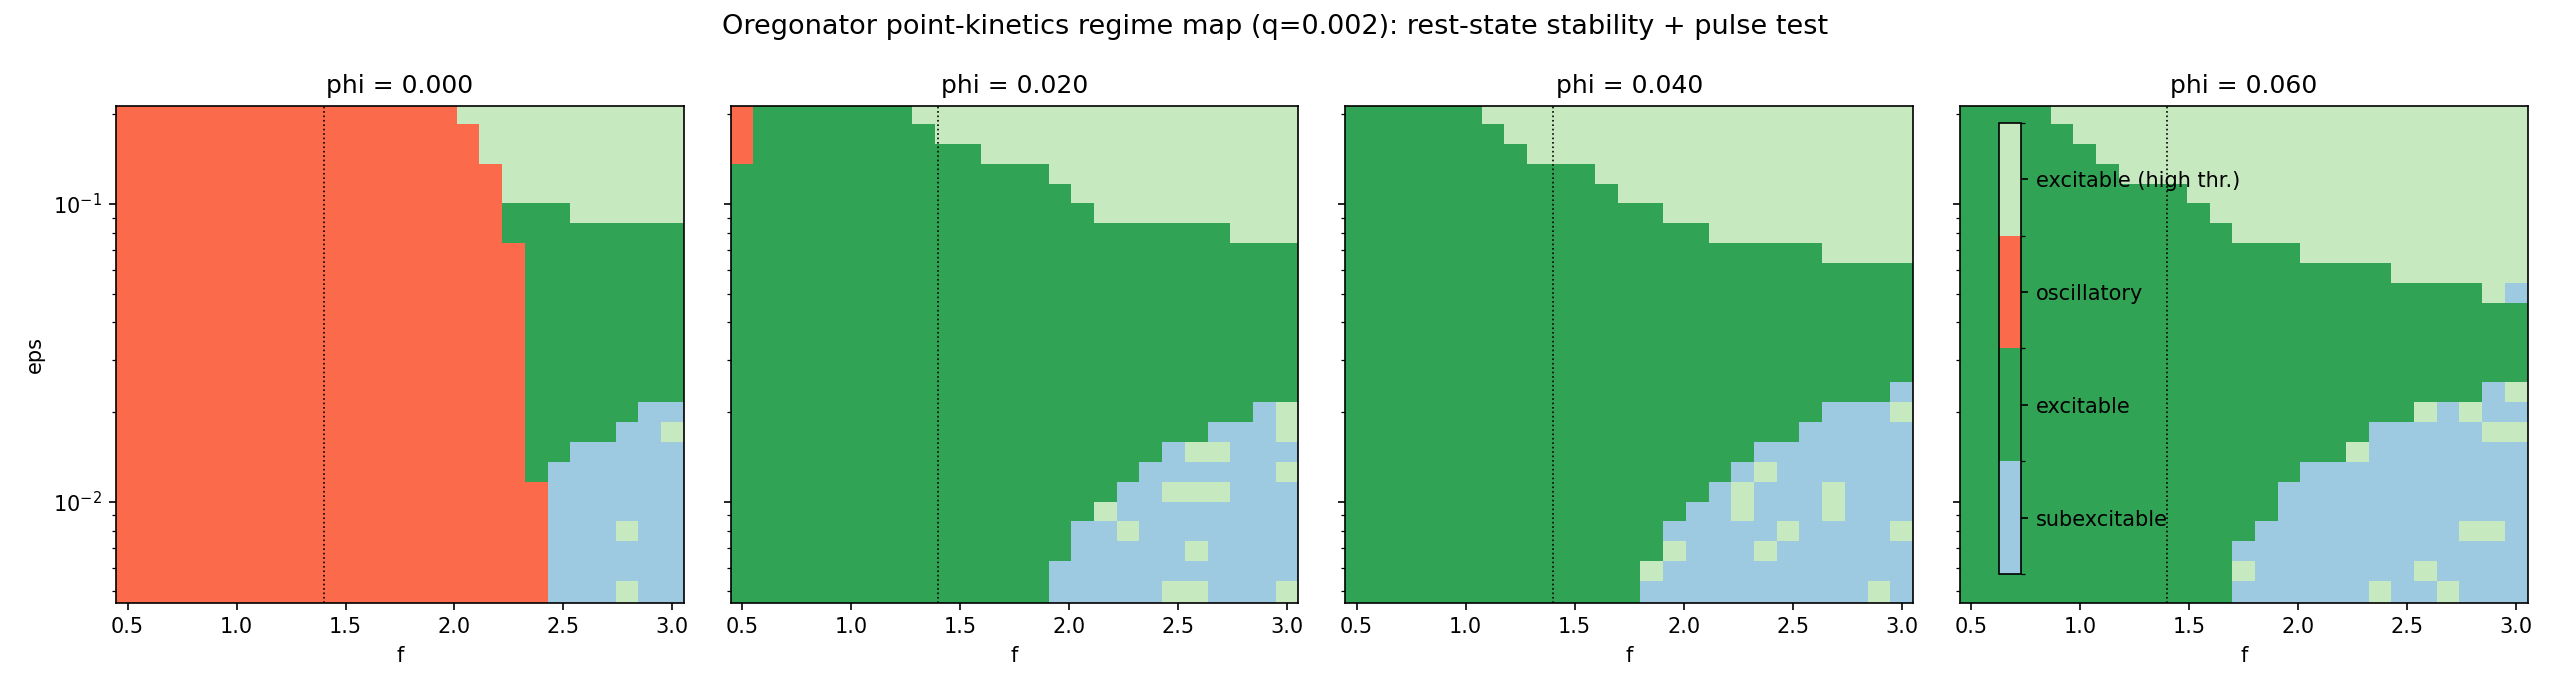
\includegraphics[width=0.8\textwidth]{../Analysis/figures/oregonator_regime_map.png}}{%
[figure pending]}
\caption{Regime map of the Tyson--Fife Oregonator kinetics in the $(\varepsilon, \phi)$ plane at $f = 1.4375$, $q = 0.002$, classified by the eigenvalues of the rest-state Jacobian. Background illumination $\phi$ stabilises the rest state, converting the spontaneously oscillatory baseline medium into a stable-excitable one suitable for pulse-based computation. The two validated working points A ($\varepsilon = 0.0501$) and B ($\varepsilon = 0.0199$) at $\phi = 0.010$ are marked.}
\label{fig:regime_map}
\end{figure}

Two excitable working points were validated in full two-dimensional simulations and are used for all Oregonator measurements in this thesis: candidate A ($\varepsilon = 0.0501$, $\phi = 0.010$), supporting pulses at $6.22$ cells per time unit, and candidate B ($\varepsilon = 0.0199$, $\phi = 0.010$), supporting faster pulses at $11.70$ cells per time unit and pairing naturally with the Barkley kinetics, whose $\varepsilon = 0.02$ is nearly identical.

\reffig{fig:phi_regime_map} fixes the working $\varepsilon = 0.0501$ and sweeps only the illumination $\phi$, because $\phi$ is the control knob used for training.
The figure distinguishes three regimes, not two.
For $\phi \lesssim 0.0045$ the rest state is linearly unstable ($\max \mathrm{Re}\,\lambda > 0$): a perturbed volume re-fires spontaneously and the medium is oscillatory.
For $\phi \gtrsim 0.0045$ the rest state is stable and a finite perturbation produces a single pulse followed by recovery, so the point kinetics are excitable.
However, point excitability does not guarantee spatial propagation: above $\phi \approx 0.026$--$0.028$ a launched pulse attenuates before it can travel tens of cells.
The usable computing window is therefore the overlap of the two conditions,
\begin{equation}
0.005 \lesssim \phi \lesssim 0.026,
\label{eq:phi_window}
\end{equation}
in which the medium is both non-oscillatory and capable of supporting propagating pulses.
The working point $\phi = 0.010$ lies near the centre of this window, with rest state $u^{*} = v^{*} = 0.00308$ and stable eigenvalues.

\begin{figure}[htbp]
\centering
\IfFileExists{../Analysis/figures/pub/pub_regime_map.png}{%
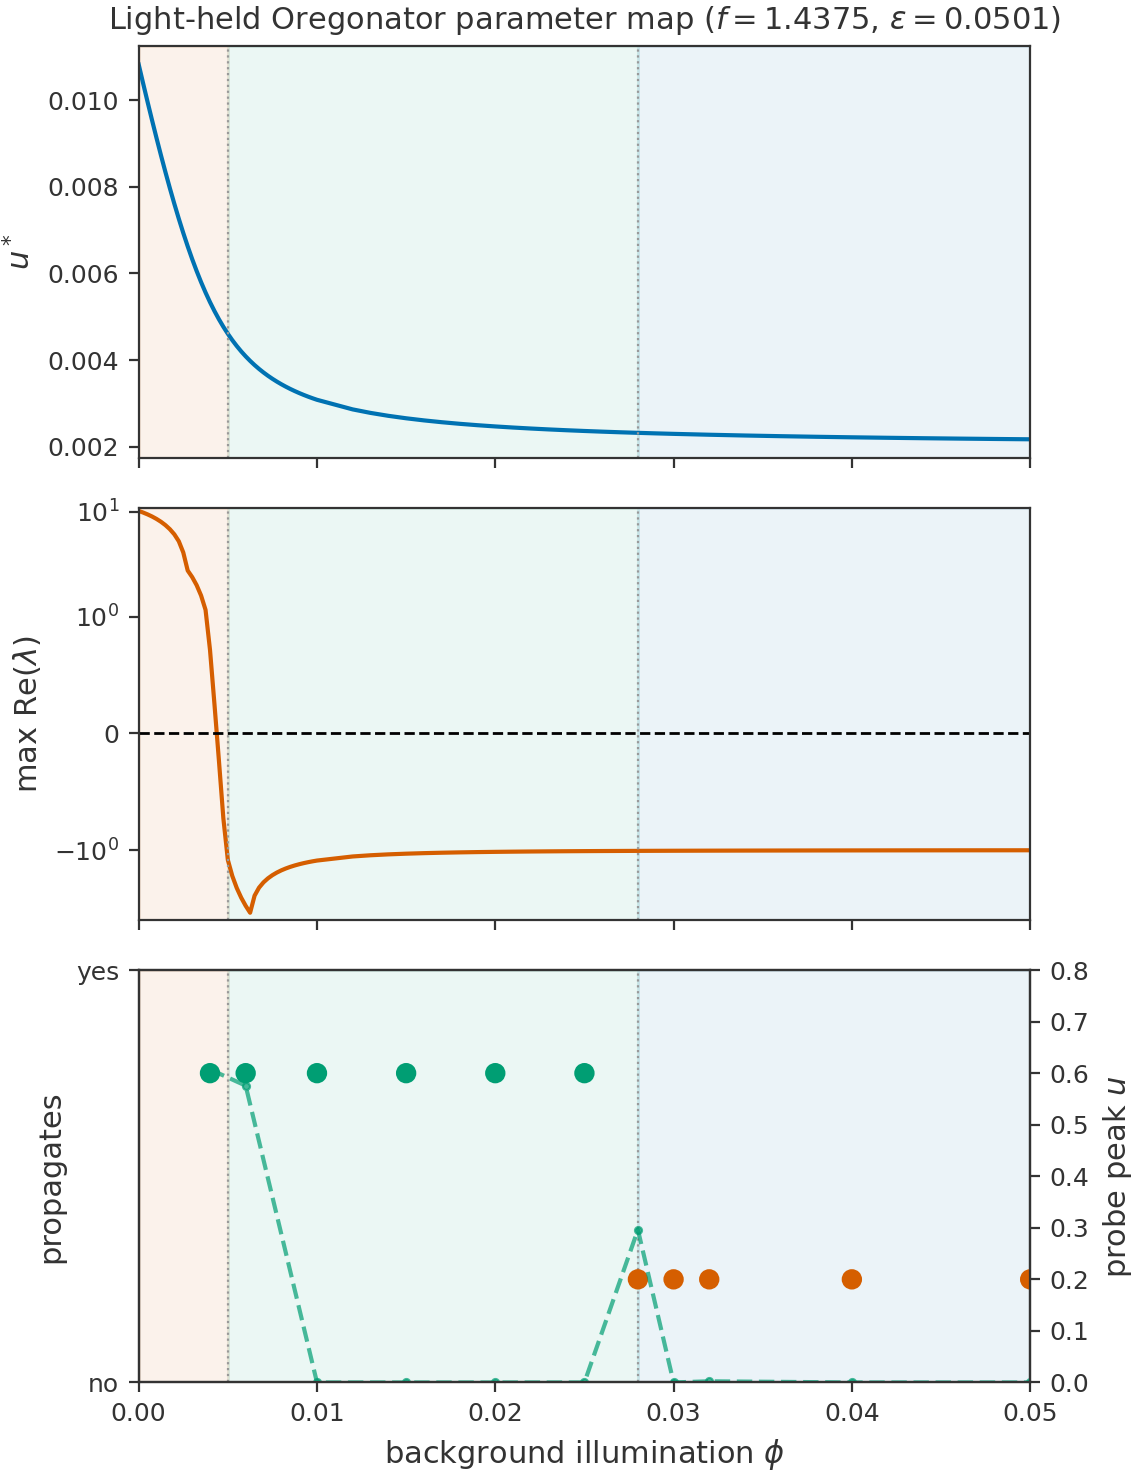
\includegraphics[width=0.85\textwidth]{../Analysis/figures/pub/pub_regime_map.png}}{%
[figure pending]}
\caption{Light-held Oregonator parameter map at the working parameters $f = 1.4375$, $\varepsilon = 0.0501$, $q = 0.002$.
Top: rest state $u^{*}$ versus background illumination $\phi$.
Middle: maximum real part of the rest-state Jacobian eigenvalues; the zero crossing marks the oscillatory--excitable boundary.
Bottom: spatial propagation flag from channel tests (green: pulse crosses $\sim$40 cells; red: it does not) and probe peak amplitude.
The usable computing window is $\phi \in [0.005, 0.026]$, shaded green: below this the medium oscillates; above it the medium is too strongly suppressed to propagate pulses.
The working point $\phi = 0.010$ is marked by the vertical grey line.}
\label{fig:phi_regime_map}
\end{figure}

One practical subtlety proved important: with $\phi > 0$ the rest state $(u^{*}, v^{*})$ of \refeqn{eq:oregonator_u}-\refeqn{eq:oregonator_v} is shifted away from the origin, so every simulation must be initialised at the numerically computed rest state rather than at $(0,0)$. Initialising at the origin amounts to applying a finite perturbation everywhere at once and contaminates the measurement before it begins.

\section{Numerical Solver and Verification}
\label{sec:meth_solver}

\subsection{Discretisation}
\label{sec:meth_discretisation}

The governing equations are discretised on a regular two-dimensional Cartesian grid with spacing $\Delta x = 1$ cell, integrated forward in time with an explicit scheme at a nominal time step $\Delta t = 0.05$ time units.
The diffusion term is discretised in divergence (flux) form: fluxes are computed on cell faces using face-averaged diffusion tensors and central differences of the field, then diverged back onto cell centres.
This form handles the anisotropic tensor field of \refSec{sec:meth_anisotropy} without special cases, and reduces exactly to the standard five-point Laplacian when the tensor is isotropic, $\mathbf{D} = D_{u}\mathbf{I}$.
No-flux walls are enforced at the flux level rather than by modifying field values: fluxes on wall-adjacent faces are set identically to zero. This conserves the diffusing species exactly and makes a wall cell behave as a true impermeable boundary rather than a damped or clipped region.
The diffusion stability constraint for an explicit two-dimensional scheme, $D\,\Delta t / \Delta x^{2} \leq 1/4$, is comfortably satisfied at the working resolution ($D_{u} = 1$ gives $0.05 \leq 0.25$).

The fast activator kinetics are the stiff part of the problem: at the working time step, $\Delta t/\varepsilon$ is $2.5$ for the Barkley model and of order unity for the Oregonator, well outside the stability region of a single forward-Euler reaction step.
Time integration therefore uses first-order operator splitting - one diffusion step followed by reaction - with the reaction stage advanced by \emph{adaptive subcycling}.
Within each outer step, the reaction substep $h$ is chosen pointwise from the analytic Jacobian of the kinetics: $h \leq 0.5 / \max(-\partial F/\partial u,\,0)$, bounding the local explicit-Euler amplification factor of the fastest contracting mode. A relative-accuracy limit $h \leq 0.1 / \max|\mathrm{d}u/\mathrm{d}t|$ and an absolute step-size limiter preventing $u$ from being pushed below $-q/2$, where the rational term $(u-q)/(u+q)$ of the Oregonator becomes singular in behaviour, complete the rule.
A NaN/Inf tripwire aborts any run in which a field leaves the finite range, so that numerical failure is always loud rather than silently absorbed.

The adaptive rule is a necessity rather than a refinement: the Oregonator's recovery-manifold Jacobian reaches approximately $-7000$ during the fast upstroke, far stiffer than any fixed explicit substep count can absorb.
The subcycled reaction stage was validated against \texttt{scipy}'s LSODA integrator, with agreement of order $10^{-6}$ on the slow phases of the excitation cycle.

\subsection{Verification Cases}
\label{sec:meth_verification}

The solver was verified against the canonical phenomenology of two-dimensional excitable media before any characterisation measurement was trusted: radially expanding target waves from a point stimulus, head-on collision of two pulses followed by annihilation, diffraction of a pulse through a gap in an occluding wall, and timing control of pulse emission.
Quantitatively, verification rested on convergence rather than on matching single runs.
Grid refinement at $\Delta x = 1$, $0.5$, and $0.25$ cells and timestep refinement about the working step $\Delta t = 0.05$ were applied to the plane-pulse speed, the physical quantity of interest underlying every transfer-function measurement.
The full convergence study, including the pre-asymptotic Barkley refinement sequence and its Richardson extrapolation, is reported in \refSec{sec:res_verification}.
The spatial deficit identified there is carried openly: all measurements reported in \refChap{chap:results} share the working resolution ($\Delta x = 1$, $\Delta t = 0.05$), so they are internally consistent as relative transfer-function measurements, and the absolute Barkley spatial deficit is stated as an explicit error bar wherever absolute speeds are quoted.

Finally, a set of runtime invariants - the NaN/Inf tripwire, the step-size guard, and the physical bounds of both fields - was monitored in every reported simulation as a guard against silent numerical corruption; the outcomes are reported with the verification suite in \refSec{sec:res_verification}.
The adaptive subcycling behaves as intended: the substep count stays at one on the slow recovery manifold and peaks at $155$ substeps within a single outer step during the firing excursion, exactly where the analytic Jacobian predicts the stiffness to lie.

\section{Substrate Parameterisation}
\label{sec:meth_parameterisation}

A computing substrate is only useful if something about it can be changed - if it exposes structure that can play the role of weights.
This substrate exposes three physically distinct parameterisations, described in the following subsections: the binary wall geometry, the graded light-suppression field $\phi(x,y)$, and the anisotropic diffusion tensor field $\mathbf{D}(x,y)$.
All three enter the same solver (\refSec{sec:meth_solver}) without modification to its core loop, and all three have direct experimental counterparts in structured and photosensitive BZ media \cite{sakurai2002design, steinbock1995anisotropy}.

\subsection{Wall Geometry}
\label{sec:meth_walls}

Walls are represented as a boolean mask on the computational grid: masked cells are impermeable, and the no-flux condition is enforced by zeroing diffusive fluxes on every wall-adjacent face (\refSec{sec:meth_discretisation}).
Walls are the coarsest and most intuitive substrate knob, a binary geometric parameterisation defining the input ports, the channels that carry pulses between them, and the junctions where pulses collide, annihilate, or diffract.
In the collision-computing tradition reviewed in \refSec{sec:lit_chemical}, the wall geometry is effectively the entire program \cite{toth1995logic, adamatzky2002xor}. In the present framework it is one of three parameterisations, and the one whose discrete, non-differentiable nature most strongly motivates gradient-free, black-box characterisation.

\subsection{Light-Suppression Field}
\label{sec:meth_light}

The light-suppression field $\phi(x,y)$ enters the activator equation through the term $(f v + \phi)(u-q)/(u+q)$ in \refeqn{eq:oregonator_u}: locally increasing $\phi$ raises the effective threshold and slows the excitable dynamics, exactly as illumination suppresses excitability in the photosensitive ruthenium-catalysed BZ reaction \cite{sakurai2002design}.
The field plays a dual role in this thesis.
Globally, a uniform background value of $\phi$ sets the operating regime of the medium; it is the knob that converts the oscillatory baseline into the stable-excitable substrate of \refSec{sec:meth_regime}.
Locally, spatial modulation of $\phi$ about that background is a graded, rewritable substrate parameterisation: brighter regions transmit pulses more slowly or not at all, so a light pattern can sculpt channels, barriers, and delays without any physical wall.
Unlike the binary wall mask, $\phi(x,y)$ is continuous-valued and experimentally rewritable in real time by a projected light pattern, which makes it the most plausible trainable knob for any future closed-loop optimisation.

\subsection{Anisotropic Diffusion Tensor}
\label{sec:meth_anisotropy}

The third parameterisation replaces the scalar activator diffusivity with a symmetric positive-definite tensor field, so that the diffusion term of \refeqn{eq:oregonator_u} becomes $\nabla\!\cdot\!(\mathbf{D}(x,y)\,\nabla u)$ with the divergence-form discretisation of \refSec{sec:meth_discretisation}.
The tensor is parameterised by its two eigenvalues $D_{\parallel} \geq D_{\perp} > 0$ and a fibre-direction field $\theta(x,y)$ giving the orientation of the fast axis.
The physical motivation is twofold: anisotropic excitable media are realisable experimentally by patterning the catalyst or printing oriented microstructure \cite{steinbock1995anisotropy}, and eikonal-curvature theory predicts a definite, testable signature - the pulse speed along the fast axis exceeds that along the slow axis by a factor $\sqrt{r}$, where $r = D_{\parallel}/D_{\perp}$ \cite{keener1991eikonal}.
Anisotropy thus offers a routing knob that neither walls nor light provide: it steers propagation direction continuously, in the interior of the medium, without blocking it.
The explicit diffusion stability constraint tightens accordingly to $D_{\parallel}\,\Delta t/\Delta x^{2} \leq 1/4$, using the largest eigenvalue of the tensor field.

\section{Black-Box Characterisation Protocol}
\label{sec:meth_protocol}

All four experiments share a single measurement protocol, designed so that the substrate is treated strictly as a black box.
Inputs are applied at \emph{ports}: small fixed regions of the grid where the activator is driven above the threshold for a fixed duration, either as a single \texttt{fire} event (one pulse) or as a \texttt{pulse\_train} (a periodic train at a prescribed frequency).
Outputs are recorded at \emph{probes}: fixed locations storing the mean activator value $u(t)$ over a small mask, yielding time series from which arrival times, amplitudes, and transmission booleans are extracted.
The internal state of the medium away from ports and probes is never inspected for the purpose of a measurement; every reported result is an input-output transfer function in the sense of \refSec{sec:meth_overview}.
Every simulation is initialised at the rest state $(u^{*}, v^{*})$ appropriate to the working $\phi$ (\refSec{sec:meth_regime}), and each experiment includes a rest-initialised no-stimulus control run, which must show zero probe activity. This checks that the medium is genuinely excitable and that no spontaneous firing contaminates the measurement.
Two input encodings are used in this thesis: the clamped-port drive above is retained for the four transfer-function experiments of \refSec{sec:meth_experiments}, while the training-era experiments of \refSec{sec:meth_demux} use the dark-spot drive described in \refSec{sec:meth_darkspot}, the experimentally honest encoding for a photosensitive medium.

One protocol decision requires justification: probe readouts are evaluated within defined time windows rather than over the whole record.
The reason is physical. At an open junction, an incoming pulse diffracts into \emph{all} connected branches, so a naive whole-record readout at a downstream probe fires whenever \emph{either} input fires - it computes OR, regardless of what the junction was designed to do.
The computation of interest lives in the collision: when both inputs arrive within the coincidence interval, their pulses annihilate and the output branch stays silent.
The probe record is therefore read within a window aligned to the expected collision outcome, isolating the annihilation event from the unconditional diffraction background.
This windowed-readout construction follows the logic of the T-shaped coincidence detectors and collision gates of the excitable-media literature \cite{gorecka2003tshaped, toth1995logic}. The window widths are set from the measured pulse speeds and refractory times of the same substrate, so the protocol is calibrated on the substrate's own dynamics rather than imposed from outside.

\subsection{Dark-Spot Input Encoding and Source Calibration}
\label{sec:meth_darkspot}

The dark-spot drive replaces the activator clamp with a one-shot flash of darkness: a local, temporary reduction of the light field within a circular spot.
The mechanism follows directly from the regime structure of \refSec{sec:meth_regime}.
The background illumination $\phi = 0.010$ holds the medium stably excitable; dimming a patch to $\phi = 0.002$ carries it across the regime boundary into the locally oscillatory regime, so for as long as the flash lasts the patch acts as a pacemaker, emitting pulses into the surrounding excitable medium.
This is the experimentally honest drive for the photosensitive ruthenium-catalysed BZ reaction, in which projected illumination is the control variable available in the laboratory \cite{sakurai2002design}: no concentration is ever clamped by hand.

The firing threshold was measured by holding patches at a range of fixed dimming levels and recording the pulse emission rate at a downstream probe (\reffig{fig:meth_darkspot}).
Emission begins at about 60\% dimming of the background suppression: patches held at $\phi = 0.006$ stay silent, while patches at $\phi = 0.004$ or darker emit full-amplitude pulses, with the emission rate rising monotonely as the dimming deepens.

\begin{figure}[htbp]
\centering
\IfFileExists{../Analysis/figures/rd_darkspot.png}{%
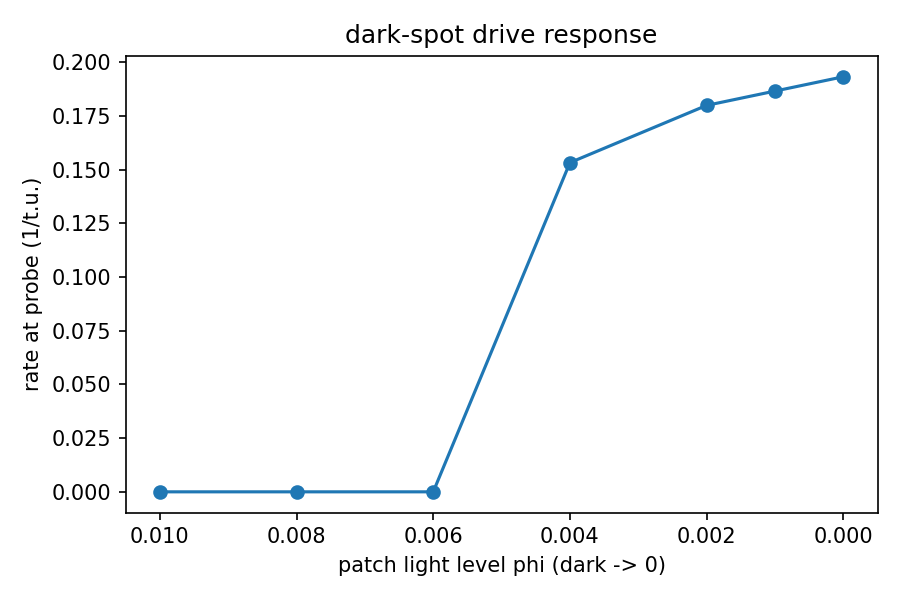
\includegraphics[width=0.7\textwidth]{../Analysis/figures/rd_darkspot.png}}{%
[figure pending]}
\caption{Dark-spot drive response. Circular patches are held at fixed light levels below the background $\phi = 0.010$, and the pulse emission rate is recorded at a downstream probe. Emission is absent down to $\phi = 0.006$ and switches on between $\phi = 0.006$ and $\phi = 0.004$ (about 60\% dimming); above threshold the rate rises monotonely with dimming depth.}
\label{fig:meth_darkspot}
\end{figure}

A dark patch is a pacemaker for as long as it is dark, so the flash duration $T_{\mathrm{flash}}$ controls how many pulses a single input event emits and must be calibrated on the medium's own dynamics.
\reftab{tab:meth_flash_calib} reports the calibration: flashes of $T_{\mathrm{flash}} \leq 4$ time units emit exactly one full-amplitude pulse (peak activator 0.709), while longer flashes emit short pulse trains spaced by the refractory time.
The first-arrival latency decreases with flash duration, from 8.7 time units for a one-unit flash to 1.7 time units for an eight-unit flash, because a longer pacemaker drive launches its first pulse earlier relative to the flash onset.
Single-pulse experiments use the operating point $T_{\mathrm{flash}} = 3.0$ time units, comfortably inside the single-pulse plateau.

\begin{table}[htbp]
\centering
\caption{Dark-spot source calibration: pulses emitted, first-arrival time at a downstream probe, and probe peak activator amplitude, as a function of flash duration $T_{\mathrm{flash}}$. Flashes up to 4 time units emit exactly one full-amplitude pulse; longer flashes emit pulse trains.}
\label{tab:meth_flash_calib}
\begin{tabular}{cccc}
\toprule
$T_{\mathrm{flash}}$ (time units) & Pulses emitted & First arrival (time units) & Probe peak \\
\midrule
1 & 1 & 8.7 & 0.709 \\
2 & 1 & 7.7 & 0.709 \\
3 & 1 & 6.7 & 0.709 \\
4 & 1 & 5.7 & 0.709 \\
6 & 2 & 3.7 & 0.709 \\
8 & 2 & 1.7 & 0.709 \\
12 & 2 & 3.8 & 0.705 \\
\bottomrule
\end{tabular}
\end{table}

\subsection{Formal Test-Case Definitions}
\label{sec:meth_testcases}

The four transfer-function experiments share a common set of controlled conditions, stated here so that every measurement is reproducible.
All simulations begin from the kinetic rest state: $u = v = 0.0030821$ everywhere for the Oregonator at $\phi = 0.010$ (the Barkley rest state is $(0,0)$ and is used only as a cross-check).
All domain boundaries and all wall cells impose a no-flux (homogeneous Neumann) condition on both $u$ and $v$, enforced at the flux level in the solver (\refSec{sec:meth_discretisation}).
The input is a clamped-port drive that holds the port cells at $u = 0.8$, $v = 0.2$ for 30 solver steps ($1.5$ time units), after which the port is released and returns to the rest state.

\textbf{Channel pulse transfer} (\texttt{rd\_transfer\_channel\_final2.py}).
Domain $256 \times 256$ cells; a straight horizontal channel of width $W$ is cut through an otherwise solid wall.
The input port is a slab at the left edge, $x \in [0,18)$, spanning the full channel width.
Three probes record mean $u$ over 3-cell vertical strips at $x = 64$ (near), $x = 128$ (mid), and $x = 217$ (far), restricted to the channel interior.
Each run lasts $2500$ steps ($125$ time units), long enough for the pulse to reach the far probe and for any post-pulse transients to decay.
A free-medium reference uses the same port geometry with no walls; a no-stimulus control confirms the medium remains at rest.

\textbf{Frequency response} (\texttt{rd\_transfer\_frequency\_final2.py}).
Domain $300 \times 48$ cells; a single horizontal channel of width $W = 16$ cells.
Input port at the left edge, $x \in [0,18)$, spanning the channel; far probe as a 3-cell vertical strip at $x = 240$.
The two-pulse refractory scan fires pairs of pulses with separations from $1$ to $32$ time units, each followed by a $1400$-step ($70$ time-unit) quiet tail.
Sustained-train runs fire six pulses at prescribed periods and record the number of threshold crossings at the far probe; the total run length is $(n_{\mathrm{pulses}}-1)P + 30 + 1400$ steps.
A no-stimulus control and a single-pulse check are run before any measurement.

\textbf{Two-input collision logic} (\texttt{rd\_transfer\_logic\_final2.py}).
The geometry is a T-junction: a horizontal channel of width $W = 20$ cells with a second channel entering from the top.
The Oregonator domain is $256 \times 200$ cells; input port A is at $x \in [25,43)$ on the horizontal channel, and input port B is at $y \in [140,158)$ on the vertical arm, centred at the junction $x = 96$.
The output probe is a 3-cell vertical strip at $x = 240$ on the horizontal channel.
Each run lasts $1000$ steps ($50$ time units) for the Oregonator ($1600$ steps for Barkley).
The truth table is evaluated from the probe peak inside a window of half-width $2.5$ time units around the expected arrival time of a lone A pulse; a delay sweep of input B measures the coincidence window for annihilation.

\textbf{Anisotropic substrate} (\texttt{rd\_transfer\_aniso\_final2.py}).
Domain $256 \times 256$ cells; no walls or ports.
The medium is initialised at rest and a circular perturbation of radius $25$ cells is seeded at the centre with $u = 0.8$, $v = 0.2$ (the same perturbation amplitude as the port drive).
A uniform anisotropic diffusion tensor with eigenvalues $D_{\parallel} = r$ and $D_{\perp} = 1$ is applied, with the fast axis aligned to $x$.
Front extents along $+x$ and $+y$ are recorded every 10 steps; run lengths are $900$, $700$, and $500$ steps for $r = 1$, $2$, and $4$, respectively.
A no-stimulus control with $r = 4$ confirms the anisotropic medium stays at rest.

These four characterisation experiments all use the clamped-port drive because it gives repeatable, model-agnostic timing and amplitude measurements.
The training-era T-junction experiments of \refSec{sec:meth_demux} use the dark-spot drive (\refSec{sec:meth_darkspot}), the experimentally honest input encoding for a photosensitive BZ layer.

\section{The Four Experiments}
\label{sec:meth_experiments}

\subsection{Channel Pulse Transfer}
\label{sec:meth_exp_channel}


The first experiment characterises the substrate's most primitive component: a wire.
A straight channel of fixed width is cut between two parallel walls, a single pulse is injected at the input port, and a probe at the far end records the arrival.
Four quantities are measured: the propagation speed in the channel, from port-to-probe delay over a known path length;
the delay linearity, confirming that travel time grows linearly with channel length so that speed is a well-defined constant of the medium;
the transmission behaviour as the channel width is swept, locating the width-induced wave-block threshold below which lateral confinement and front curvature extinguish the pulse;
and, around that threshold, the sharpness of the transition from transmission to block.
The results are reported in \refSec{sec:res_channel}.

\subsection{Frequency Response}
\label{sec:meth_exp_frequency}

The second experiment measures the substrate's bandwidth, which is set by refractoriness: behind every pulse lies a zone that cannot be re-excited until the recovery variable has decayed, so a channel acts as a low-pass device for pulse trains.
A pulse train of prescribed frequency is injected at the input port and the probe records which pulses transmit.
The experiment is run in two forms: a two-pulse measurement, in which the interval between two successive pulses is swept to locate the absolute refractory period directly; and a sustained-train measurement, in which the output frequency $f_{\mathrm{out}}$ is recorded against the input frequency $f_{\mathrm{in}}$, giving the transmission ratio curve and the maximum 1:1 following rate above which pulses begin to be dropped.
The results are reported in \refSec{sec:res_frequency}.

\subsection{Two-Input Collision Logic}
\label{sec:meth_exp_logic}

The third experiment measures the substrate's native logic.
Two input channels converge on a T-junction, with probes on the output branch downstream of the collision region. The two inputs, A and B, are each either pulse-present or pulse-absent, giving the four input combinations of a two-input truth table.
With the windowed readout of \refSec{sec:meth_protocol}, the probe record is converted into truth-table entries: lone pulses that reach the junction propagate or diffract onward, while coincident pulses collide, annihilate, and leave the output silent.
Three figures of merit are measured: the truth table itself at each probe; the separation ratio between the weakest ``true'' output signal and the strongest ``false'' one, which quantifies the noise margin of the gate; and the inhibition window - the range of relative input timings within which the trailing pulse is still annihilated - which quantifies the gate's tolerance to clock skew.
The results are reported in \refSec{sec:res_logic}.

\subsection{Anisotropic Substrate}
\label{sec:meth_exp_anisotropy}

The fourth experiment characterises the anisotropic parameterisation of \refSec{sec:meth_anisotropy}.
In a uniform tensor field with anisotropy ratio $r = D_{\parallel}/D_{\perp}$, a point stimulus is fired and the expanding pulse is tracked. The $\sqrt{r}$ eikonal law of \refSec{sec:meth_anisotropy} - elliptical fronts whose axis ratio and fast-to-slow speed ratio both scale as $\sqrt{r}$ - provides a direct quantitative check of the tensor discretisation.
The directional speed profile $c(\theta)$ is measured by probing along rays at several orientations to the fibre direction.
Finally, a patch of anisotropic medium embedded in the isotropic substrate is used to measure how propagation delay across the patch depends on the orientation of its fibres relative to the incident wave direction - the routing signature that anisotropy adds to the design space beyond walls and light.
The results are reported in \refSec{sec:res_anisotropy}.

\section{Uncertainty Quantification Protocol}
\label{sec:meth_uq}

To make the characterisation trustworthy, the uncertainty in the measured transfer functions must be quantified.
The forward solver is deterministic, but the Oregonator kinetic parameters and the background illumination are not known exactly in any real experiment.
A variance-based sensitivity analysis propagates this parameter uncertainty to the channel-pulse quality of interest.

The quantities of interest are the pulse speed $c$ between two small centre-line probes in a straight channel and the peak activator value $u_{\mathrm{peak}}$ recorded at the downstream probe.
Four scalar parameters are treated as independent uniform random variables, each varied by $\pm 10\%$ around the working point:
\begin{itemize}
    \item $\varepsilon$ (activator/recovery timescale separation),
    \item $f$ (stoichiometric factor),
    \item $\phi$ (uniform background light-suppression field),
    \item $D_{u}$ (isotropic activator diffusivity).
\end{itemize}
The diffusion tensor is kept isotropic here; the anisotropic-routing experiment of \refSec{sec:meth_exp_anisotropy} is analysed separately.

A one-at-a-time sensitivity sweep is used instead of a full variance-based decomposition, because the forward solve is expensive and the qualitative ranking is sufficient for a first uncertainty-quantification pass.
Each of the four parameters is varied independently by $\pm 10\%$ around its nominal value while the others are held fixed, giving nine additional channel-pulse solves.
The resulting percentage change in pulse speed and probe peak is recorded for each parameter \cite{abbaszadeh2019uncertainty}.
A run is discarded if the homogeneous rest state is unstable at the sampled parameter set; in practice all sampled points remained inside the stable-excitable window.

\section{Training Protocol: T-Junction Directionality Routing}
\label{sec:meth_demux}

The experiments of \refSec{sec:meth_experiments} characterise a fixed substrate; the final methodological step closes the loop and trains the substrate for a routing task.
A full demultiplexer geometry (V5, \reffig{fig:meth_demux_geometry}) was prepared as the eventual target, but its first optimisation campaign did not converge within the available budget, so the training proof-of-concept reported here uses a simpler T-junction directionality task.

\subsection{Prepared Geometry: Demultiplexer V5}
\label{sec:meth_demux_geometry}

The geometry, designated V5 and frozen before training began, is a $200 \times 200$ cell free medium with no walls (\reffig{fig:meth_demux_geometry}).
Two circular input spots of radius 12 cells sit at A$(40, 80)$ and B$(40, 120)$.
Six probes record the response: PC$(95, 100)$ near the centre of the routing region, and five output probes PA1$(82, 26)$, PA2$(114, 58)$, PA3$(125, 100)$, PA4$(114, 142)$, and PA5$(82, 174)$ fanning out downstream of it.
Only PA1, PA3, and PA5 carry assignments; the unassigned probes exist so that misrouted pulses are counted rather than lost.
The trainable region is the rectangle $x \in [55, 135]$, $y \in [20, 180]$, parameterised by an $8 \times 8$ bilinear control grid with 64 parameters bounded to $\phi \in [0.010, 0.025]$.
Circular halos of radius 10 cells around every probe are pinned to the background value.
Inputs are one-shot dark flashes, $\phi = 0.002$ held for 12 time units on the flashed spots (\refSec{sec:meth_darkspot}).
This geometry and loss were prepared for future work; the results reported in \refSec{sec:res_tjunc_train} use the simpler T-junction described below.

\begin{figure}[htbp]
\centering
\IfFileExists{../Analysis/figures/rd_demux_geometry_v5.png}{%
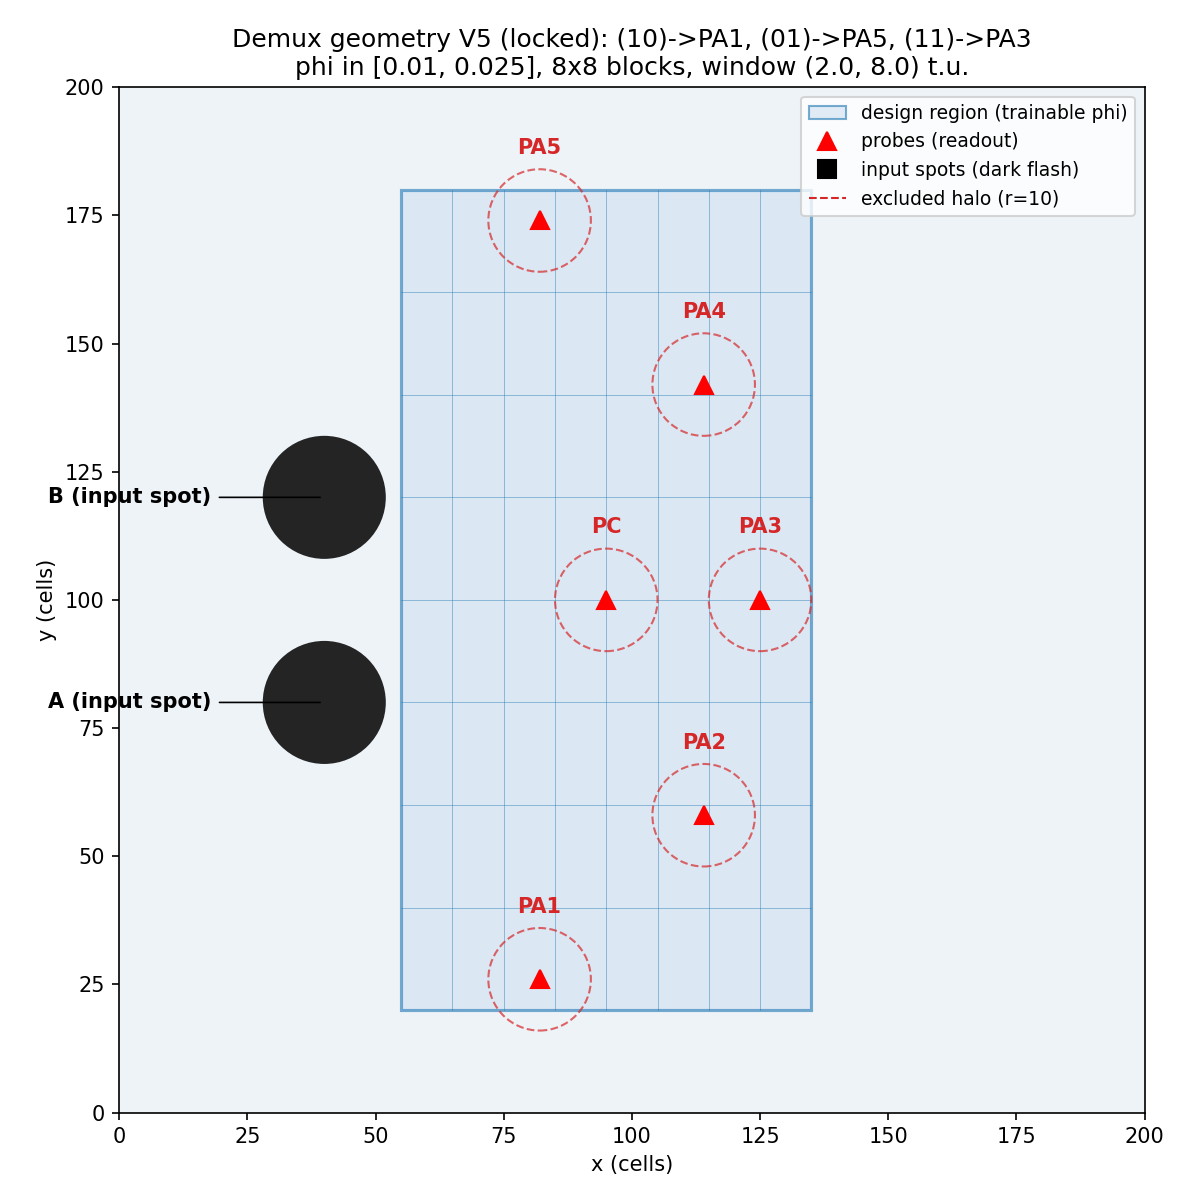
\includegraphics[width=0.7\textwidth]{../Analysis/figures/rd_demux_geometry_v5.png}}{%
[figure pending]}
\caption{Demultiplexer training geometry V5, prepared for future work. Input spots A and B (radius 12 cells) receive one-shot dark flashes; probes PC and PA1 to PA5 record arrivals. The shaded rectangle is the trainable region, tiled by the $8 \times 8$ control grid; dashed circles mark the probe halos pinned to the background light level. Assigned routes: (10) to PA1, (01) to PA5, (11) to PA3.}
\label{fig:meth_demux_geometry}
\end{figure}

\subsection{T-Junction Directionality Task}
\label{sec:meth_tjunc_task}

The reported training task is single-input directionality routing in a fixed-wall T-junction.
A vertical stem feeds a horizontal bar; a one-shot dark-spot flash at the base of the stem launches a single pulse into the junction.
The objective is to make the pulse reach one assigned output probe while the opposite output probe remains below threshold; the mirrored task (route to the other output) is also solved.
Probes record the spatial maximum of $u$ over a small disk, because the mean over the disk is diluted by the wake and underestimates the wavefront amplitude at a T-junction.

The light field $\phi(x,y)$ around the junction is parameterised by a $4 \times 4$ bilinear interpolation grid, giving 16 continuous parameters bounded to $\phi \in [0.010, 0.040]$.
The lower bound is the excitable background and the upper bound lies above the propagation-blocking level measured in \refSec{sec:res_phi_window}, so the optimiser can choose either to let pulses pass or to suppress them locally.

\subsection{Loss Function and Optimiser Comparison}
\label{sec:meth_demux_loss}

Two objectives are recorded for each candidate field.
The soft objective penalises a low peak at the assigned output and a high peak at the wrong output:
\begin{equation}
L_{\mathrm{soft}} = (1 - u_{\mathrm{assigned}}) + u_{\mathrm{wrong}},
\label{eq:tjunc_soft_loss}
\end{equation}
where $u_{\mathrm{assigned}}$ and $u_{\mathrm{wrong}}$ are the probe maxima inside the readout window, normalised so that the ideal field gives zero loss.
The hard objective records whether the assigned probe crosses the threshold $u = 0.5$ while the wrong probe does not.

Four gradient-free optimisers are compared on a small budget of expensive forward evaluations: random search, differential evolution (DE), dual annealing, and CMA-ES.
Each candidate evaluation runs a fresh, rest-initialised simulation of the T-junction on the candidate field and returns both objectives.
The comparison identifies which algorithm is best able to discover the correlated block pattern that suppresses one branch without extinguishing the pulse, before the full demultiplexer task is attempted.
